\begin{figure}[tb]
\centering
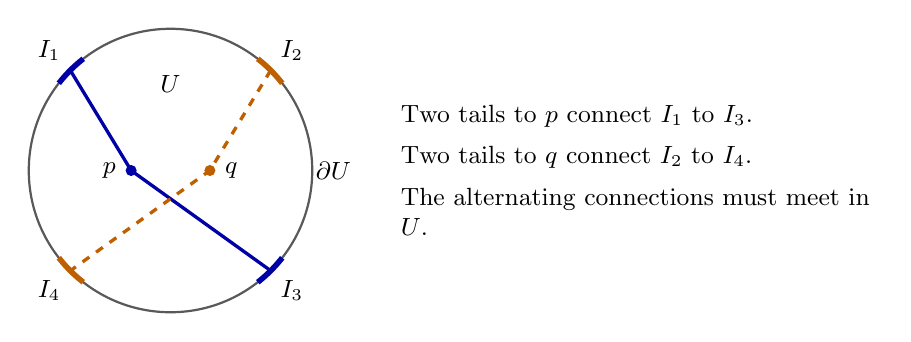
\begin{tikzpicture}[x=1cm,y=1cm,font=\small]
 \draw[black!65,line width=.8pt] (0,0) circle (1.8);
 \draw[blue!65!black,line width=2pt]
 (128:1.8) arc[start angle=128,end angle=142,radius=1.8];
 \draw[orange!75!black,line width=2pt]
 (38:1.8) arc[start angle=38,end angle=52,radius=1.8];
 \draw[blue!65!black,line width=2pt]
 (308:1.8) arc[start angle=308,end angle=322,radius=1.8];
 \draw[orange!75!black,line width=2pt]
 (218:1.8) arc[start angle=218,end angle=232,radius=1.8];
 \node at (2.07,0) {$\partial U$};
 \node at (0,1.1) {$U$};
 \draw[blue!65!black,line width=1.2pt]
 (-1.273,1.273)--(-.5,0)--(1.273,-1.273);
 \draw[orange!75!black,line width=1.2pt,dashed]
 (1.273,1.273)--(.5,0)--(-1.273,-1.273);
 \fill[blue!65!black] (-.5,0) circle (2pt);
 \fill[orange!75!black] (.5,0) circle (2pt);
 \node[left,xshift=-2pt] at (-.5,0) {$p$};
 \node[right,xshift=2pt] at (.5,0) {$q$};
 \node[above left] at (-1.273,1.273) {$I_1$};
 \node[above right] at (1.273,1.273) {$I_2$};
 \node[below right] at (1.273,-1.273) {$I_3$};
 \node[below left] at (-1.273,-1.273) {$I_4$};
 \node[align=left,text width=6cm,anchor=west] at (2.8,0)
 {Two tails to $p$ connect $I_1$ to $I_3$.\\[4pt]
  Two tails to $q$ connect $I_2$ to $I_4$.\\[4pt]
  The alternating connections must meet in $U$.};
\end{tikzpicture}
\caption{The four-path crossing in the quotient disk $U$.
The four boundary arcs occur in cyclic order. After diffuse dust
contacts have been removed, the probability of any required meeting
is bounded by the occupation and hit estimates.}
\label{fig:crossing}
\end{figure}
